\documentclass[12pt,a4paper]{article}
\usepackage[utf8]{inputenc}
 

\usepackage[comma, authoryear]{natbib}
\usepackage{graphicx}
\usepackage{url}
\usepackage{hyperref}
\usepackage{setspace}
\usepackage{float}
\usepackage{lscape}
\usepackage{pdfpages}
%\usepackage{fullpage}
\setlength{\parskip}{0.5cm plus4mm minus3mm}
% Länkformat
\hypersetup{colorlinks=false,
            urlcolor=RoyalBlue}
            
\title{Distributed product information management with Git \\ version 2}
\author{Tor Nilsson Öhrn}
\date{April 2013}

\begin{document}

% TITLEPAGE
\begin{titlepage}
\begin{center}


\textsc{\LARGE Distributed product information management with Git}\\[0.2cm]
%\emph{Master's thesis}\\[2.5cm]
\textsc{\Large Master's thesis \\ Linköpings University \\  2014}\\[0.5cm]

\begin{figure}
    \begin{center}
        
\includegraphics[scale=2.0]{images/liu_logo.png}
    \end{center}
    \vspace{1.0cm}
\end{figure}

\emph{Written by:}\\
\textsc{Tor Nilsson Öhrn}\\
tornilssonohrn@gmail.com\\[0.5cm]

\end{center}
\end{titlepage}

%----------------------------- Innehålls-, figur- och tabellförteckning
\tableofcontents
\addtocontents{toc}{\protect\thispagestyle{empty}}
\clearpage

\setcounter{page}{1}

\clearpage 

\begin{abstract}
In this thesis it is evaluated how the version control system Git can be used for product information management in a distributed manner. Running Git on smart-phones empowers customers to participate in collaboration with manufacturers and resellers in the creation and management of product information throughout the life of a product.

\end{abstract}

\section{Introduction}
Traditionally only manufacturers and resellers of products have had the tools to create, track and manage product information. Scanners and IT-systems are used to keep track of products until they finally reach their end users. Customers have been referring to a manufacturer or reseller's website when looking for information about their bought products.

\subsection{Motivation}
Today many consumers are equipped with smart-phones that have networking, media and NFC features, allowing them to perform product information management previously reserved for larger manufacturers and resellers. Also as the market for second hand products grows, consumers are often becoming resellers themselves which poses new challenges for how product information should be stored and managed. There is for example currently no prevailing way of transferring information about a product between manufacturers, resellers, customers and second hand customers. 

\subsection{Purpose}
Our ambition is to propose a solution for distributed product information management based on the version control system Git. By setting up a working demonstration of this new concept that simulates a test case we hope to convince the reader that this is a viable solution. Questions that we will try to answer are for example:
\begin{itemize}
  \item How well suited is Git to be used as the foundation of a product lifecycle management (PLM) systems?
  \item How could Git be customized to better meet to the requirements of a PLM system?
\end{itemize} 

\subsection{Limitations}
This thesis will not provide a fully functional implementation of a PIM system. The consumer facing side of the proof of concept will only be implemented to run on the Android mobile OS and will assume that the device supports NFC. The Android application implemented in this thesis has only been tested to run as just-in-time compiled code on the Dalvik Runtime and not with the ahead-of-time compilation used by the newer Android Runtime. It is also assumed that the reader of this thesis knows basic Git terminology and workflow.


\section{Theory}


\subsection{Product Information}
\label{productinformation}
Product information can be separated into two major categories, type specific product information (TSPI) and item specific product information (ISPI). Manufacturers and resellers would mostly contribute with TSPI such as technical specifications and manuals whereas the customer would provide ISPI such as images and damage reports of the specific item they have bought. 

Kary Främling et al. have found that ISPI would need to be stored in a back-end system rather than in the product itself \citep{gupi}. They also conclude that the product needs to be uniquely identifiable among other products and that one have to take into consideration that the product will only have limited internet access. These are all challenges that we will take into consideration when Git is evaluated as a tool for PIM. 

% methods to identify products
Currently there exists a few competing standards for uniquely identifying products. For this thesis the so called ID@URI method used by the DIALOG system from the Helsinki university of technology has been chosen because it makes use of already existing open standards and is simple in its structure compared to its competitors \citep{gupi}. Främling et al. writes that the ID@URI approach creates a globally unique product identifier (GUPI) by combining an URI, which preferably can consist of an URL which uniqueness is guaranteed by the already existing Domain Name System, with an ID that is unique for that URL \citep{agentbased}. 

The back-end system that handles PIM can be set up in a centralized or a decentralized manner and there are different pros and cons of both. Corcelle et al. states that any realistic item-level PIM system must be at least partially distributed \citep{isim}. 

\subsection{Git}
Git is, according to Susan Potter \citep{osa}, not limited to only represent source code. She states that `It (Git) supports distributed workflows, allowing a body of work to either eventually converge or temporarily diverge.` If we assume the digital body of work to be product information this type of workflow might look like the one depicted in \emph{Figure \ref{fig:workflow}}. 

\begin{figure}[!ht]
    \centering
    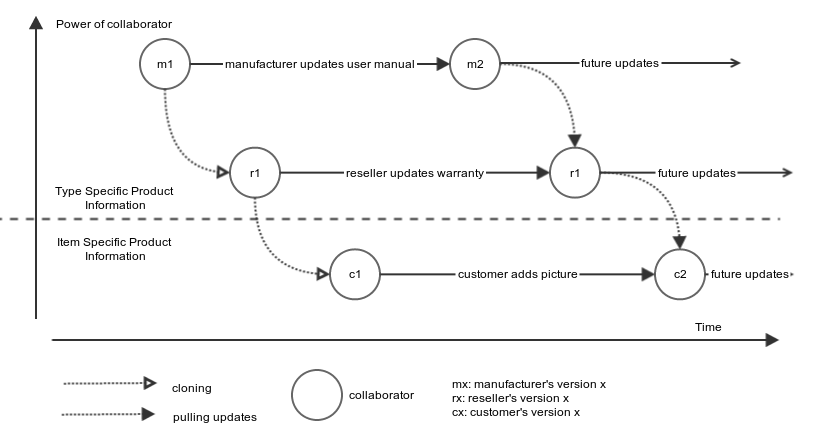
\includegraphics[scale=0.4]{images/workflow2.png}
    \caption{Product information as a diverging and converging body of work shared between different collaborators }
    \label{fig:workflow}
\end{figure}



\subsubsection{storage}
The object database that Git relies on represents any type of files that are organized in a classic file hierarchy as a directed acyclic graph (DAG) \citep{progit}. An example of this can be seen in \emph{Figure \ref{fig:storage}}.

\begin{figure}[!ht]
    \centering
    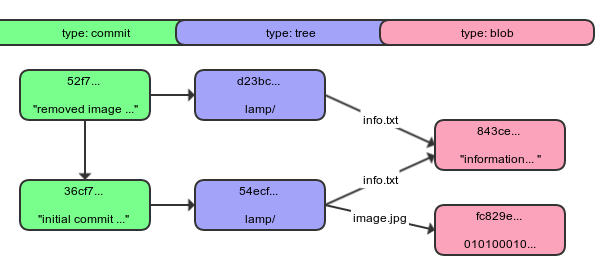
\includegraphics[scale=0.5]{images/storage.png}
    \caption{How git represents the version control of a file hierarchy}
    \label{fig:storage}
\end{figure}

Each file and folder stored in this DAG is represented by its SHA-1 checksum which makes it infeasable to change or corrupt files without Git knowing about it. The DAG also reuses an old version of a file if that file's checksum has not changed since the last commit, an example of which is the file \emph{info.txt} in \emph{Figure \ref{fig:shallowclone}}.

The distributed nature of Git makes it store a full copy of the object database on each collaborators system. All files are by default compressed with Zlib's LZ77 type compression, something which already compressed, like jpeg or png, image files won't benefit much from. For example a large image file of a product is committed but then later on deleted it will still occupy a lot of disk space. Git is generally not very well designed for managing image files since they are big blobs of binary data that diff and merge tools by default can't do much with. Since product information geared towards customers could consist of quite a few images we need to decide how Git should handle them. One way could be to let Git just store metadata about the images in the git object database and then fetch the actual imagedata from for example URLs found in the metadata. 
        
\subsubsection{repositories}
But how are we to distinguish between TSPI and ISPI with Git? This is not something that Git was designed for but the ID@URI method discussed in the \nameref{productinformation} section happens to map pretty well to a git backend system. In this thesis the URI part of the ID@URI will consist of an URL to a remote git repository containing the TSPI. This TSPI repository is assumed to be managed by a manufacturer or reseller of a product. The TSPI repository is then very much like a normal Git repository where many collaborators can work together with a digital piece of work.

\subsubsection{cloning}
The ISPI is different to what Git usually deals with since it represents a specific instance of the product, i.e a certain physical entity. As such it won't have the same need for supporting a traversal of the change log. Therefore a clone from a TSPI repository down to a ISPI repository can be a shallow one, i.e a clone with depth 1. The difference between a normal, deep clone, and a shallow one can be seen in \emph{Figure \ref{fig:shallowclone}}.

\begin{figure}[!ht]
    \centering
    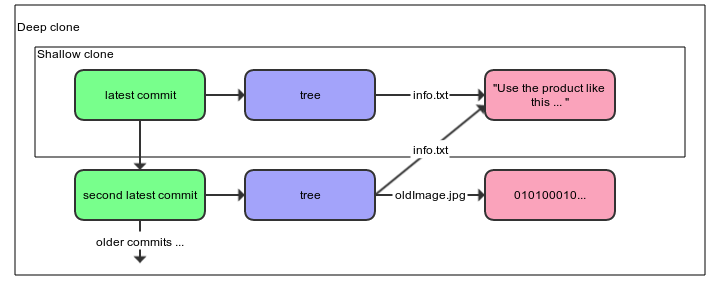
\includegraphics[scale=0.5]{images/shallow.png}
    \caption{A shallow clone occupies less space}
    \label{fig:shallowclone}
\end{figure}

\subsubsection{Data integrity}
\emph{something about the SHA-1 method used by Git, not sure if this really needs to be covered so much ...}
%\subsection{Transactions} %not sure if this should be covered, overkill?
%Satoshi Nakamoto's whitepaper about Bitcoin explains a concept of storing a transaction history as a chain of digital signatures \citep{bitcoin}. 

%The private/public key infrastructure needed for that is already used by OpenSSH which comes with Git.

\subsection{Git on Android}
Android is predicted to be the dominant OS by 2016 surpassing Windows \citep{android}, and might displace classic "embedded Linux" on non-user-centric devices which are very relevant for product information since products many times falls under this category. Android is also increasingly not only developed by Google as companies like Cyanogenmod and Linaro forks an android release and then develop their own flavor of the OS. Our choice of operating system for our PIM application to be used by the customer is therefore Android.

According to Karim Yaghmour \citep{android}, applications for the Unix based operating system Android are usually developed in Java with help from the Android Software Development Kit (SDK). The Java code of the application is then compiled to bytecode and executed with Android's Dalvik virtual machine. There are a few Git on Android applications today but they mostly uses a pure Java implementation of Git called JGit which doesn't provide much lower level features, refered to by Scott Chacon \citep{progit} as Git plumbings. Libgit2 is a linkable library implemented in C that has an API which allows to write third party custom Git applications. It comes with much of the same core functionality as Git itself as well as methods for lower level customization. To use the C methods that Libgit2 comes with on Android the application needs to make use of the Android Native Development Kit (NDK). The Android NDK uses the Java Native Interface (JNI) to communicate between platform independent Java bytecode and platform dependent compiled native code written in for example C. How methods from a native C library like LibGit2 is called in an Android application can be seen in \emph{Figure not yet created ...}. 


\subsection{RFID}
Främling et al. writes that the ID@URI GUPI method, explained in the \nameref{productinformation} section, can be implemented by embedding an ID@URL reference in a passive RFID tag \citep{gupi}. Passive RFID tags can nowadays be read and written to by an increasing number of smart-phones. As of the Autumn of 2014 Google's Android mobile OS already have support for these NFC features and the next Apple's iOS will, according to Bloomberg, also include NFC features \citep{apple}. For this thesis we have chosen to implement the test case by using a Mifare Classic 1k tag which today is in widespread use in public transport ticketing systems around the world and is supported by the Android API. The Mifare card's cryptographic read/write protection has been compromised \citep{micrack} so the data stored on the card should be assumed to be readable and writeable by an attacker.

The Mifare Classic tag needs to contain references to one or more remote repositories as well as some kind of product identifier.

\subsection{Assessment}
\label{assessment}
In order to evaluate Git as a tool for PIM we need to have some formal requirements it needs to fulfil. By conducting case studies Ranasinghe et al. \citep{plcm} have found such requirements for a product lifecycle management (PLM) system. The requirements they found, and their role in the PLM system, can be seen in Table \ref{tab:criterias}. We do not intend to quantify how well Git fulfils these requirements instead give a qualitative review in the result section of this thesis.

%different parts in the products life


\begin{table}[h]
\begin{tabular}{p{4cm}|p{10cm}}
Requirement & Role \\
\hline \\
Globally unique identifier & To provide the link between product instance and information. \\ \\
Routing or lookup mechanisms & To provide the ability to find or search for product related data \\ \\
Information Resources & For the persistent storage of life cycle data \\ \\
Timely Information & To ensure that the information system can support PLM strategies based on real-time information \\ \\
Synchronisation & To ensure data synchronicity in an environment of multiple data sources and storage locations for an individual object \\ \\
Reconfigurability & To provide robustness and interoperability between technologies, vendors and devices \\ \\
Application support & To ease the burden of creating high level PLM applications \\ \\
\end{tabular}
\caption{Requirements for a PLM system \citep{plcm}}
\label{tab:criterias}
\end{table}

\section{Method}
A minimal prototype that uses Git for PIM between a server, a smartphone and a Mifare Classic tag attached to a product was set up for the purpose of this thesis. By doing so we were able to assess how well Git fulfills the requirements listed in the \nameref{assessment} section. The activity diagram in Figure \ref{fig:activity} shows how those three entities communicated with each other.

\begin{figure}[h]
    \centering
    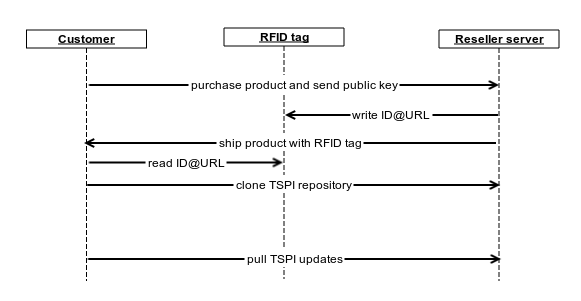
\includegraphics[scale=0.6]{images/activity.png}
    \caption{Activity diagram of the proposed implementation}
    \label{fig:activity}
\end{figure}

\subsection{Customizing Git}
Since Git can be used in so many different ways some design choices had to be taken about how it could best be used when PIM is the goal. Scott Chacon \citep{progit} describes 
\subsubsection{Storage}
\label{storage}

\subsubsection{Cloning}

\subsubsection{Merging strategies}

\subsection{Type specific information}
- A gitolite server with SSH access. 
- Customer sends their public key to be embedded in initial signature before cloning

\subsection{Item specific information}

\subsection{LibGit2}
- Mature library
- Possibility to customize git workflow
- JNI 
\subsection{Libgit2 and Android}
- OpenSSL keystore can't be found in https requests, ignore SSL check, bad fix
- SDcard's FAT32 doesn't support unix style file modes, make chmod a no-op
- Threadsafe results in error, not sure why
- 
\subsection{MifareClassic RFID tags}

- Unsafe storage, 48 bit A and B keys
- 752 bytes of storage space
Store:
- TSPI remote URL
- ID
- 

%\subsection{Transactions}
%- Bitcoin style signature chain
%- Length limitations due to very limited storage space
%- 

\section{Results}

\subsection{Globally unique identifier}
\subsection{Routing or lookup mechanisms}
Somewhat vulnerable to changing domain names for updates but distributed nature makes it strong still
\subsection{Information Resources}
\subsection{Timely Information}
\subsection{Synchronisation}
\subsection{Reconfigurability}
\subsection{Application support}

\section{Discussion}
Maybe Git is fundamentally not a good choice, do we need vc for product information? Ingenious design though. 
composite products
allows updates when user want to
Git is rather new and LibGit2 not very mature, we have yet to see creative implementations of it since git as such has a very broad and well implemented functionality. Torvalds Linux went from desktops to smartphones with Android, will Git take the same trip?
\subsection{Method}
\subsection{Result}
\subsection{Wider context}

\section{Conclusions}


\clearpage
\bibliographystyle{apalike} 
\bibliography{thesis}

\end{document}
